\documentclass[../main.tex]{subfiles}
\begin{document}
\chapter{User Guide}
\section{Installing the extension for Visual Studio Code}
The easiest way to install the extension is from Visual Studio Code. This is done by navigating to the Extensions window and searching for \codeword{NikolaiMerritt.logical-english-vscode}. The extension is hosted at \url{https://marketplace.visualstudio.com/items?itemName=NikolaiMerritt.logical-english-vscode} and can be installed from there too. Once installed, Visual Studio Code will keep the extension up to date automatically.

\section{Running the language server manually}
To run the language server manually, you will need
\begin{itemize}
    \item node (\url{https://nodejs.org/en/download/}) version 16.4.5 or newer
    \item node package manager (npm) version 8.12.2 or newer
\end{itemize}
Having downloaded the repository at \url{https://github.com/nikolaimerritt/logical-english-vscode}, navigate to the \codeword{vscode-package} directory. Run \codeword{npm install}. This installs all the node packages for the syntax highlighter, language server, and visual studio code client. 
\\
\\
To run the language server, from the \codeword{vscode-package/server} folder, run \codeword{npm link}. (You may have to run this command with super user or administrator privileges). This creates the language server as a node package called \codeword{le-server}. Test that it launches without errors by running \codeword{le-server --stdio}. This should produce no output.
\\
\\
As per the Language Server Protocol, the language server, \codeword{le-server}, listens to input from standard console input (\codeword{stdio}).

\section{Reading the source code}
The source code for the entire extension, which includes the language client, syntax highlighter and language server, can be found at \url{https://github.com/nikolaimerritt/logical-english-vscode} under the MIT license.

\section{Features Description}
\subsection{Highlighting}
\begin{figure}[h!]
\centering
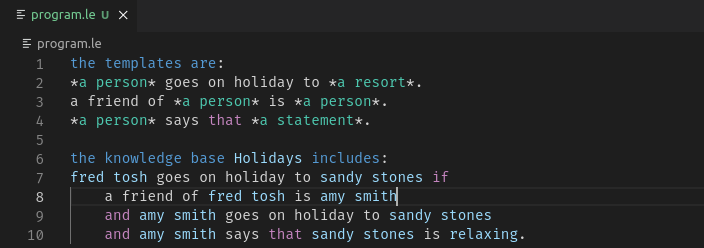
\includegraphics[width = \linewidth]{./figures/highlighting.png}
\caption{A diagram showing the overall structure of the Logical English editor.}
\label{fig:system-overview}
\end{figure}

\subsection{Code Completion}\begin{figure}[h!]
\centering
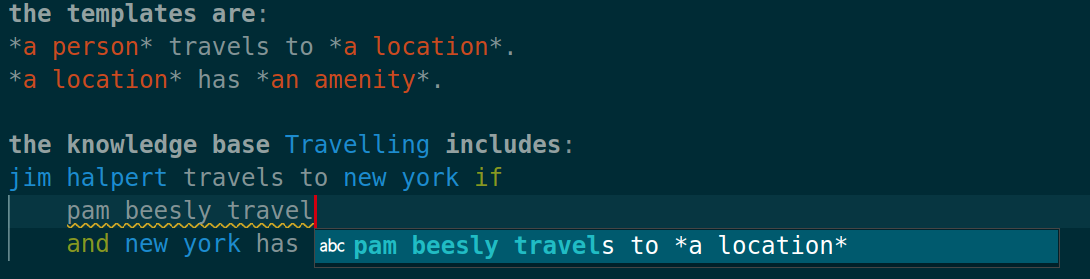
\includegraphics[width = \linewidth]{./figures/auto-suggest.png}
\caption{A diagram showing the overall structure of the Logical English editor.}
\label{fig:system-overview}
\end{figure}

\subsection{Error Diagnosis}
\begin{figure}[h!]
\centering
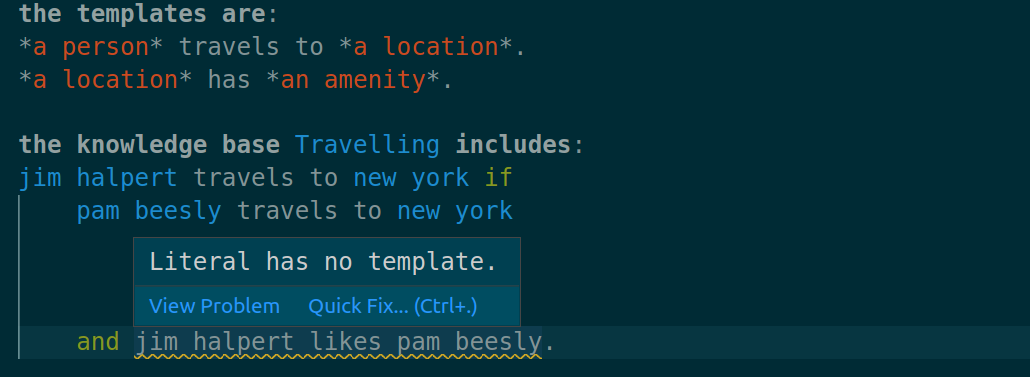
\includegraphics[width = \linewidth]{./figures/literal-wo-template.png}
\caption{A diagram showing the overall structure of the Logical English editor.}
\label{fig:system-overview}
\end{figure}

\begin{figure}[h!]
\centering
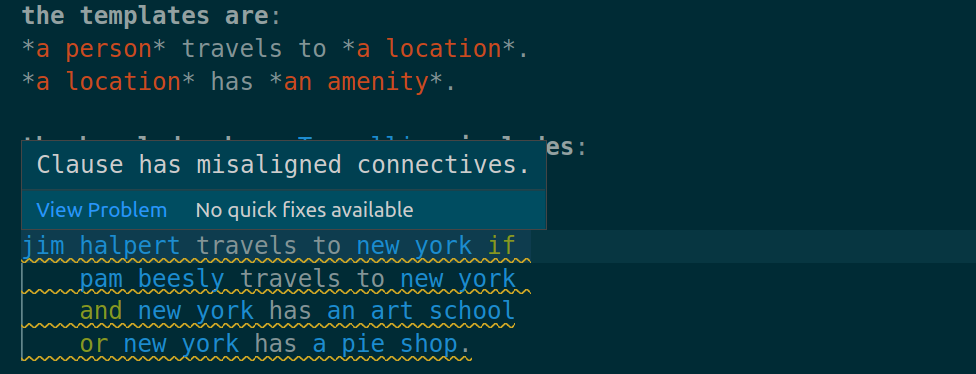
\includegraphics[width = \linewidth]{./figures/misaligned-connectives.png}
\caption{A diagram showing the overall structure of the Logical English editor.}
\label{fig:system-overview}
\end{figure}

\subsection{Code Actions}
\begin{figure}[h!]
\centering
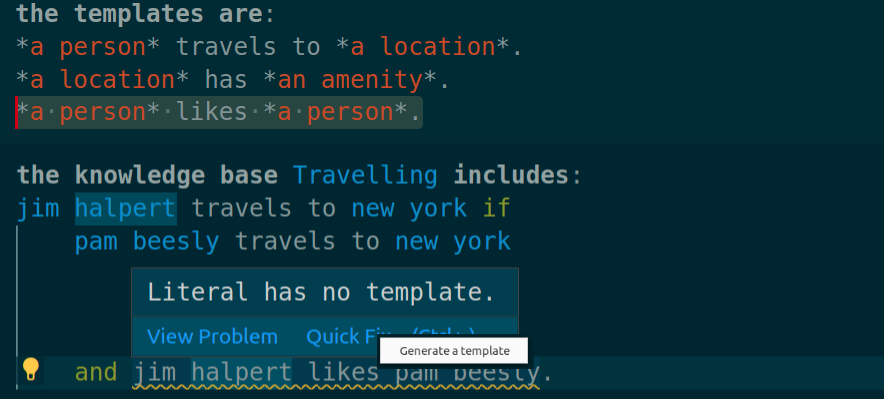
\includegraphics[width = \linewidth]{./figures/generate-template-full.png}
\caption{A diagram showing the overall structure of the Logical English editor.}
\label{fig:system-overview}
\end{figure}

\subsection{Type Checking}
\begin{figure}[h!]
\centering
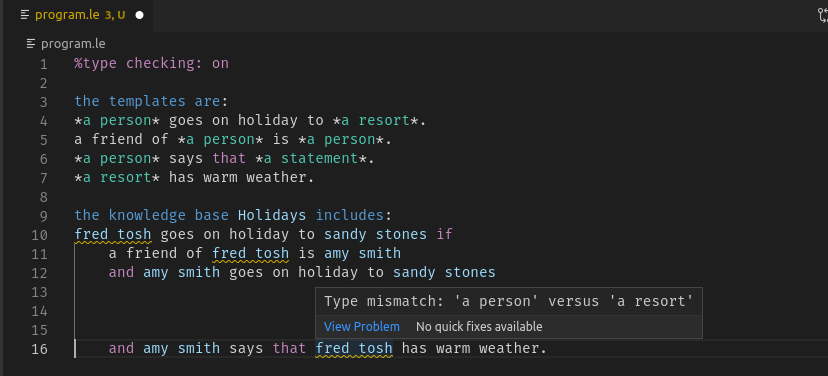
\includegraphics[width = \linewidth]{./figures/type-error.png}
\caption{A diagram showing the overall structure of the Logical English editor.}
\label{fig:system-overview}
\end{figure}

\begin{figure}[h!]
\centering
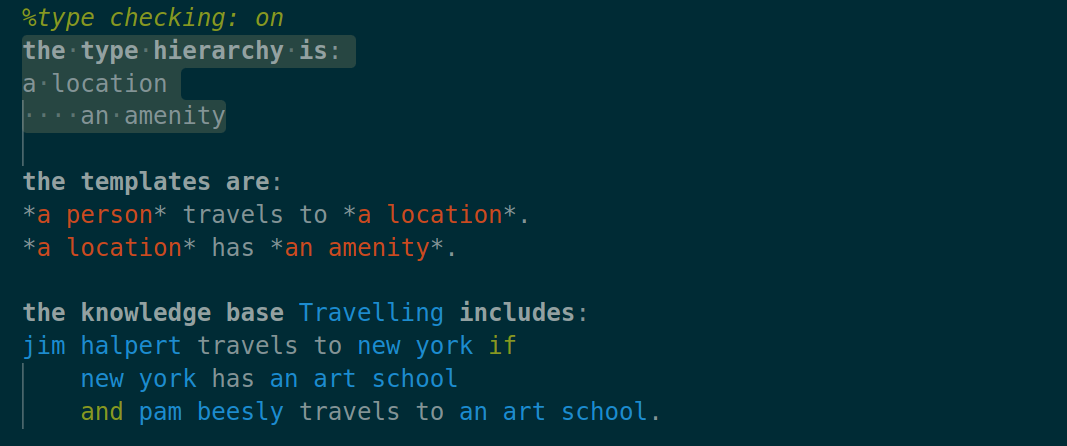
\includegraphics[width = \linewidth]{./figures/type-hierarchy.png}
\caption{A diagram showing the overall structure of the Logical English editor.}
\label{fig:system-overview}
\end{figure}
\end{document}